\documentclass{article}
\usepackage[paperwidth=13in,paperheight=15in,margin=.125in]{geometry}
\usepackage{color}
\usepackage{graphicx}
\usepackage{verbatim}
\usepackage{float}

\definecolor{bg}{RGB}{230,230,250}
\definecolor{sundriedClay}{RGB}{39,40,34}
\definecolor{violetBorder}{RGB}{98,22,141}
\pagecolor{bg}
\begin{document}
\begin{tabular}{@{}c@{} @{}c@{}}
\includegraphics[height=6in,width=6in]{SpaDis}&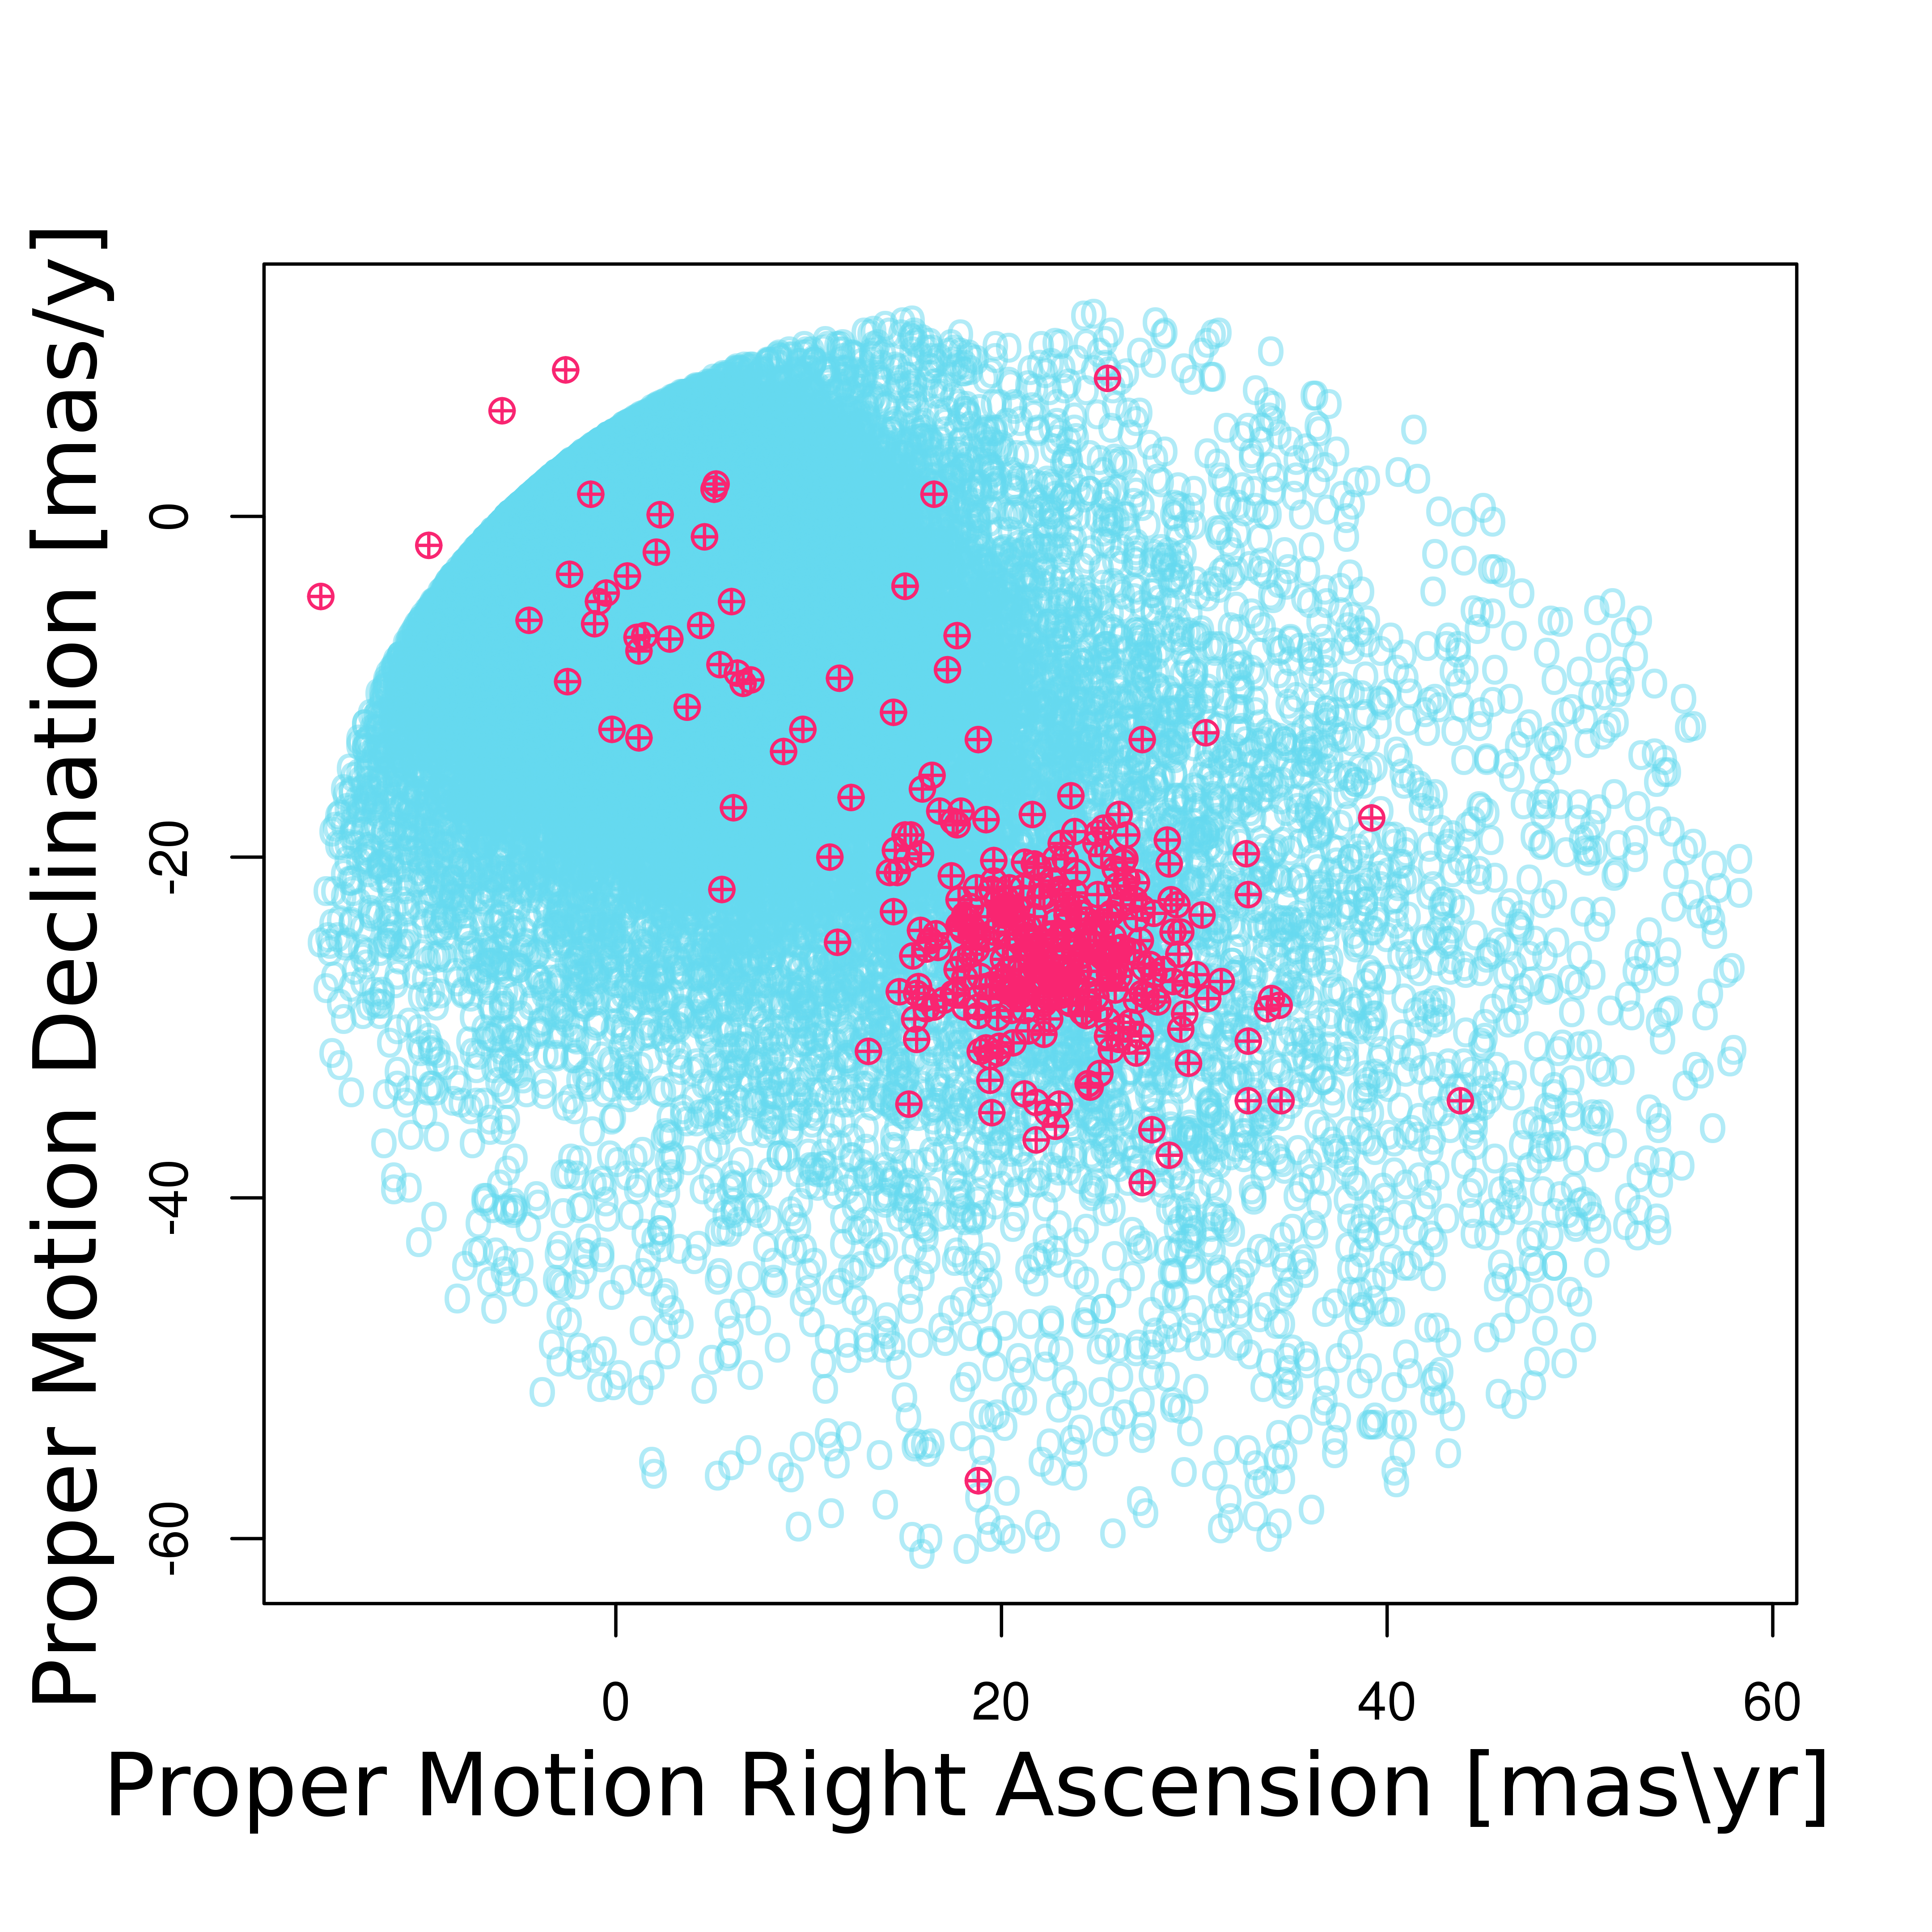
\includegraphics[height=6in,width=6in]{ProDis}\\
\large Spacial Distribution in geometric space of catalog members and known members&\large Spacial Distribution in proper motion space of catalog members and known members\\
\includegraphics[height=6in,width=6in]{SpaPro}&\includegraphics[height=6in,width=6in]{ProPro}\\
\large Membership probability versus Spacial Distance of catalog members and known members& \large Membership probability versus distance in proper motion space
\end{tabular}

%\color{violetBorder}
\setlength{\fboxsep}{0in}%
\setlength{\fboxrule}{0.375in}%
\begin{comment}
\floatstyle{boxed}{\fbox{
\begin{figure}[tl]
	\includegraphics[height=6in,width=6in]{SpaDis}
	\caption{Spacial Distribution in geometric space of catalog members and known members}
\end{figure}\begin{figure}[tr]
	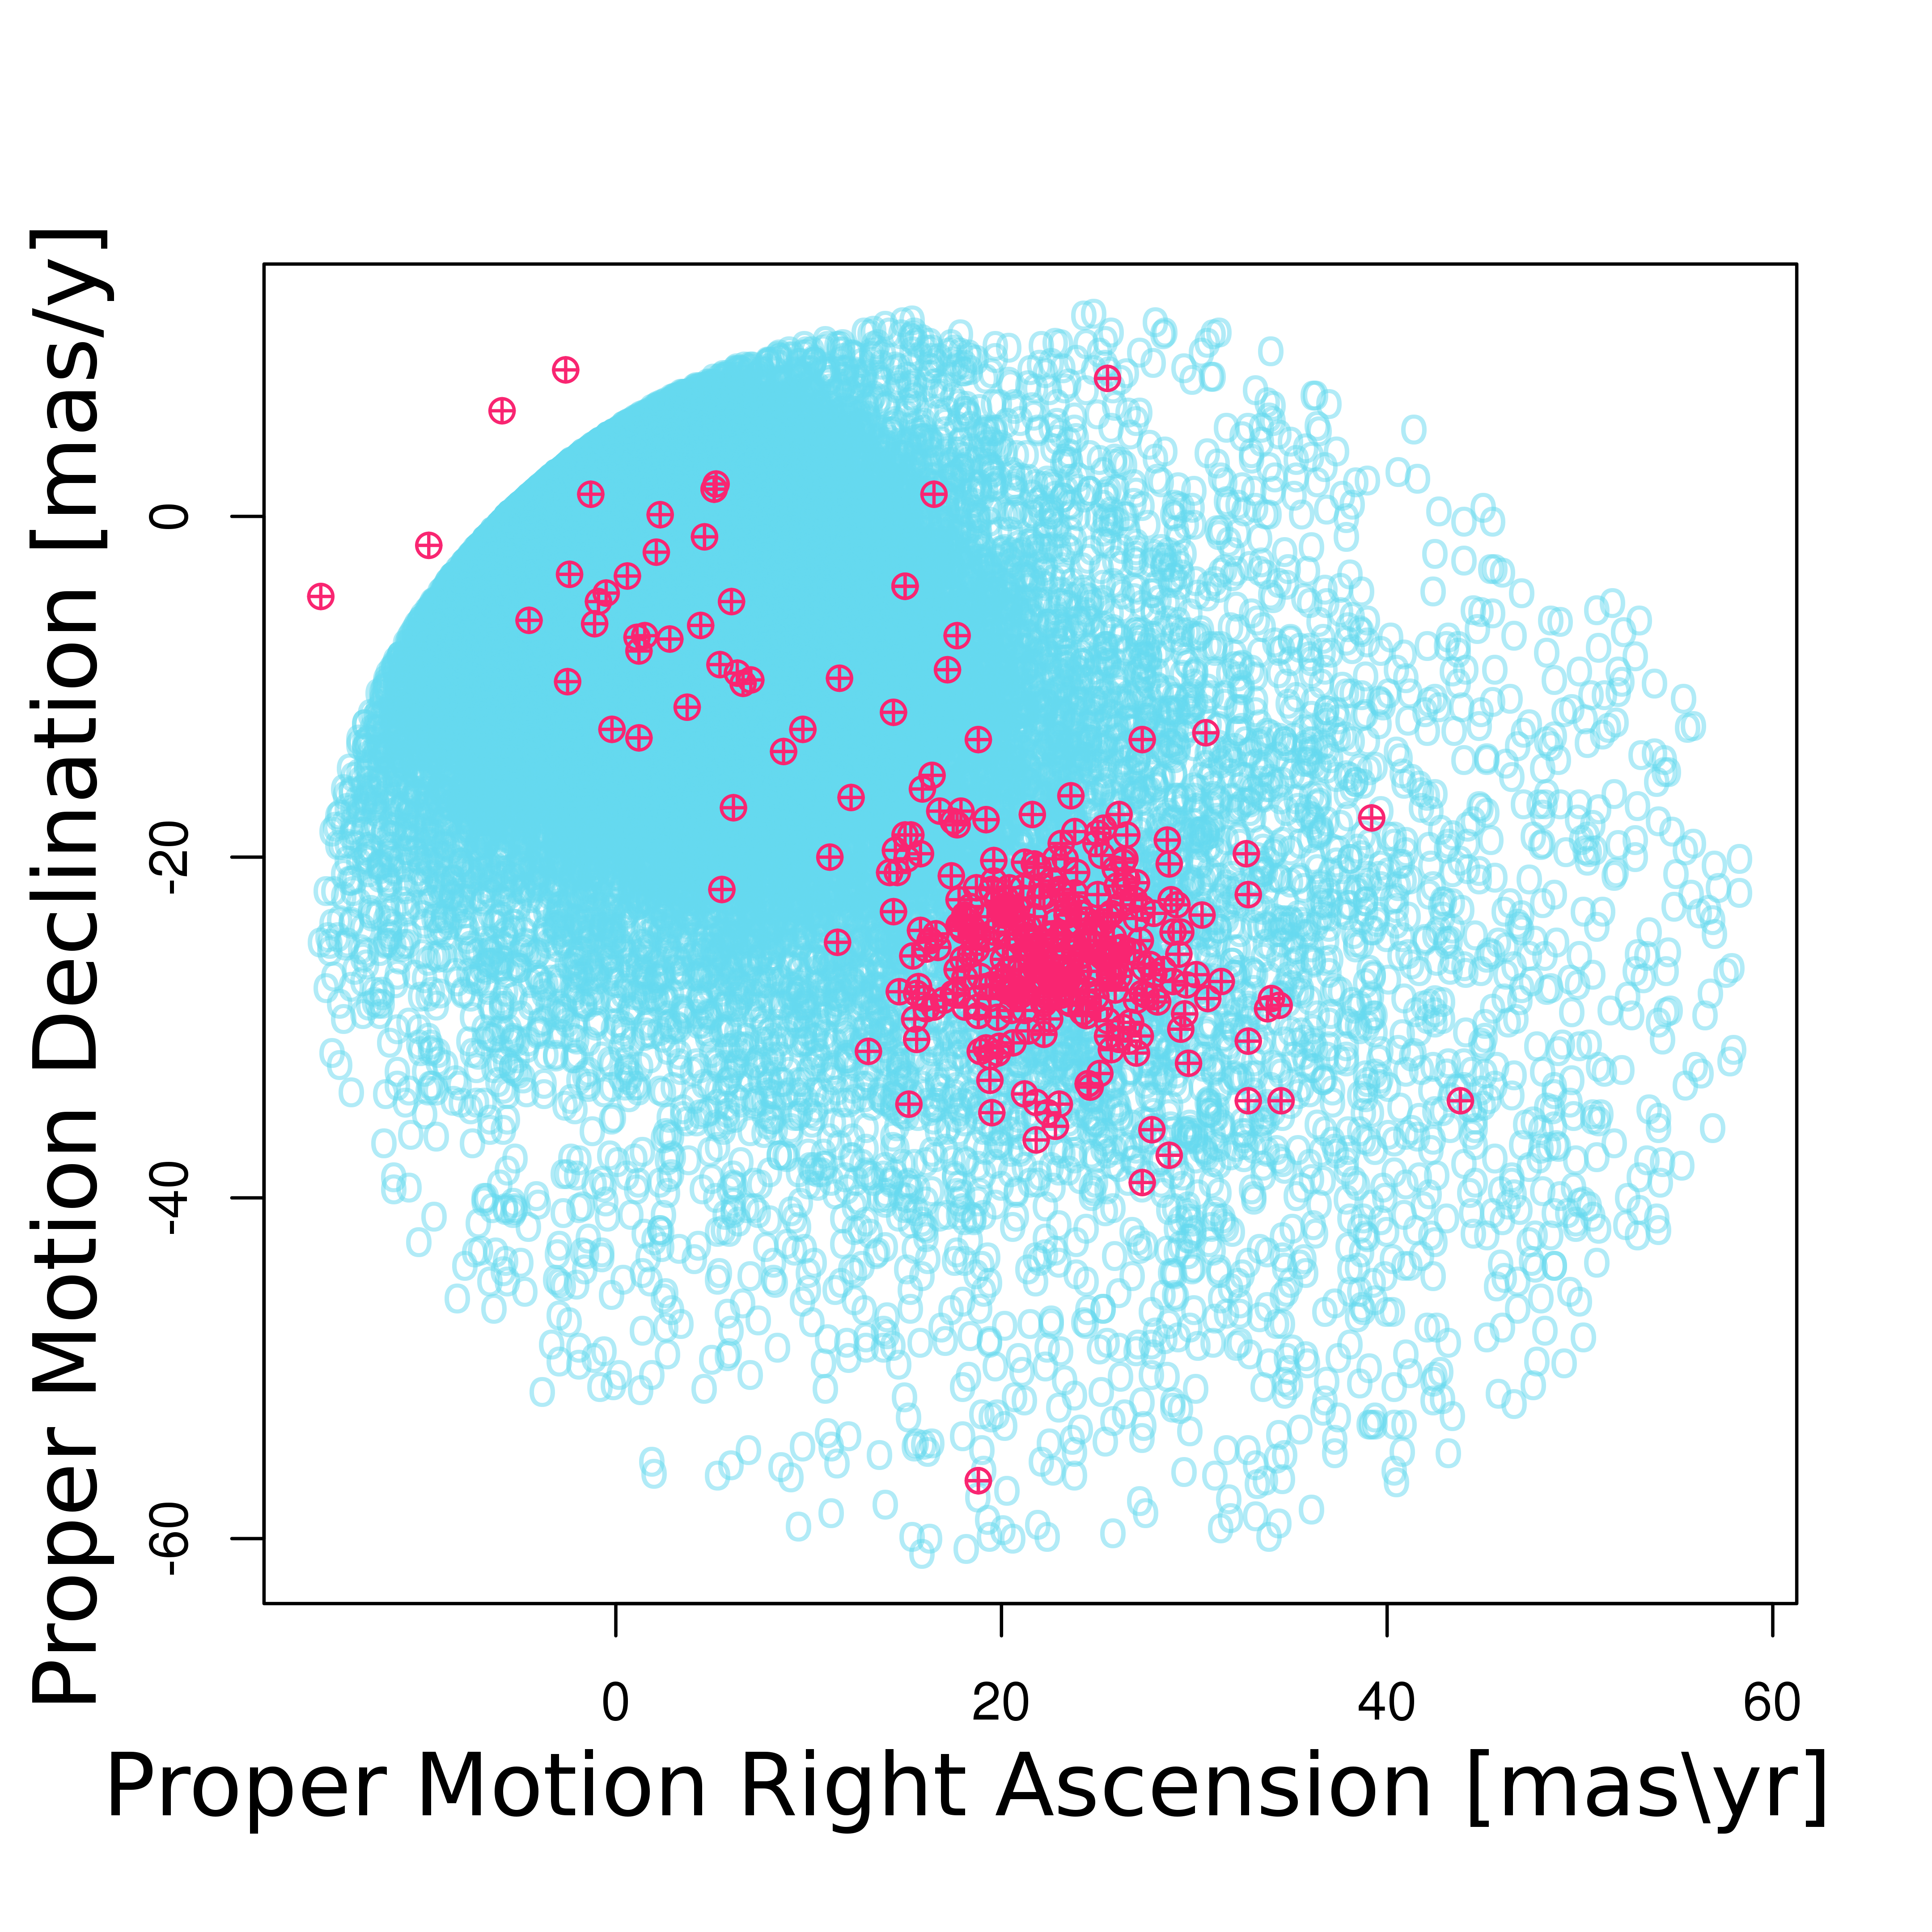
\includegraphics[height=6in,width=6in]{ProDis}
	\caption{Spacial Distribution in proper motion space of catalog members and known members}
\end{figure}
\begin{figure}[bl]
	\includegraphics[height=6in,width=6in]{SpaPro}
	\caption{Membership probability versus Spacial Distance of catalog members and known members}
\end{figure}\begin{figure}[br]
	\includegraphics[height=6in,width=6in]{ProPro}
	\caption{Membership probability versus distance in proper motion space of catalog members and known members}}}
\end{figure}
\end{comment}
\end{document}
